\subsection{Brownian Motion}
The field of stochastic systems started with an observation by Robert Brown in 1827.
In Brown’s experiment, there are two types of forces at work.\\
First, even with the particle at rest, it is bombarded by gas or fluid molecules in its surrounding.\\
Secondly, if the particle is moving, it will face more energetic collisions in the direction it is moving, and the particle will slow down.\\
This process is described at the macroscopic level by the frictional force which is exerted on a particle in a viscous fluid and leads to an acceleration opposite to the direction of its velocity.
Assuming the particle is spherical this force is given by Stoke’s law as
\begin{equation}
	\mathbf{F}=-6\pi\eta R\mathbf{v}
\end{equation}
where $\eta$ is the viscosity of the fluid and $R$ the radius of the sphere.\\
Regarding the process that leads to the movement, we have no idea what force is acting on the particle at a given time, neither its strength, nor its direction, so we simply call it $\mathbf{\tilde{\xi}}(t)$.\\
For simplicity we look at at a one-dimensional system, i.e. a particle that only moves along a line to the left or right. Then Newton’s second law can be applied:
\begin{equation}{\label{eq:bm1}}
	F=ma=-6\pi\eta rv+\tilde{\xi}(t)\quad\rightarrow\quad a=\dot{v}=-\underbrace{\frac{6\pi\eta R}{m}}_{\alpha}v+\underbrace{\frac{1}{m}\tilde{\xi}(t)}_{\xi(t)}
\end{equation}
Inserting the substitutions as indicated in (\ref{eq:bm1}) we obtain
\begin{equation}{\label{eq:bm2}}
	\dot{v}=-\alpha v+\xi(t)
\end{equation}
Equations of the form (\ref{eq:bm2}) with a deterministic part (here $-\alpha v$) and an additive stochastic part (here $\xi(t)$) are called \textbf{Langevin equations}.\\
We have always dealt with equations that are called \emph{autonomous} or \emph{homogeneous}, which means that the right-hand side does not explicitly depend on time.
Equations like (\ref{eq:bm2}) that contain such an explicit time dependence are called \emph{nonautonomous} or \emph{inhomogenous}.
\begin{theorem}
	The general solution of an \emph{inhomogeneous} differential equation is given by the the \emph{sum} of the general solution of the corresponding homogenous equation and a particular solution of the inhomogeneous equation.
\end{theorem}
According to this theorem we first have to find the general solution of the homogeneous equation,
\begin{equation}
	\dot{v}=-\alpha v\quad\rightarrow\quad v(t)=ce^{-\alpha t}
\end{equation}
Now we have to find a particular solution of the inhomogenous equation, which is done by a procedure called \emph{variation of the constant}.
The constant $c=c(t)$
\begin{equation}
	v_p(t)=c(t)e^{-\alpha t}\quad\rightarrow\quad \dot{v}_p(t)=\dot{c}(t)e^{-\alpha t}-\alpha c(t)e^{-\alpha t}
\end{equation}
which we insert into the original equation (\ref{eq:bm2}) to determine the ‘constant’ $c(t)$
\begin{equation}
	\dot{v}_p(t)=\dot{c}(t)e^{-\alpha t}-\alpha c(t)e^{-\alpha t}=-\alpha c(t)e^{-\alpha t}+\xi(t)\quad\rightarrow\quad \dot{c}(t)=\xi(t)e^{\alpha t}\quad\rightarrow\quad c(t)=\int_{-\infty}^t\xi(t^\prime)e^{\alpha t^\prime}dt^\prime
\end{equation}
Now the particular solution of the inhomogeneous equation reads
\begin{equation}{\label{eq:lesn}}
	v_p(t)=e^{-\alpha t}\int_{-\infty}^t\xi(t^\prime)e^{\alpha t^\prime}dt^\prime\quad\rightarrow\quad v(t)=ce^{-\alpha t}+e^{-\alpha t}\int_{-\infty}^t\xi(t^\prime)e^{\alpha t^\prime}dt^\prime
\end{equation}
For large $t$ the first term in (\ref{eq:lesn}) vanishes and we finally obtain
\begin{equation}{\label{eq:lesln}}
	v(t)=\int_{-\infty}^t\xi(t^\prime)e^{-\alpha(t-t^\prime)}dt^\prime
\end{equation}
\begin{figure}[H]
	\centering
	\begin{subfigure}{0.55\linewidth}
		\centering
		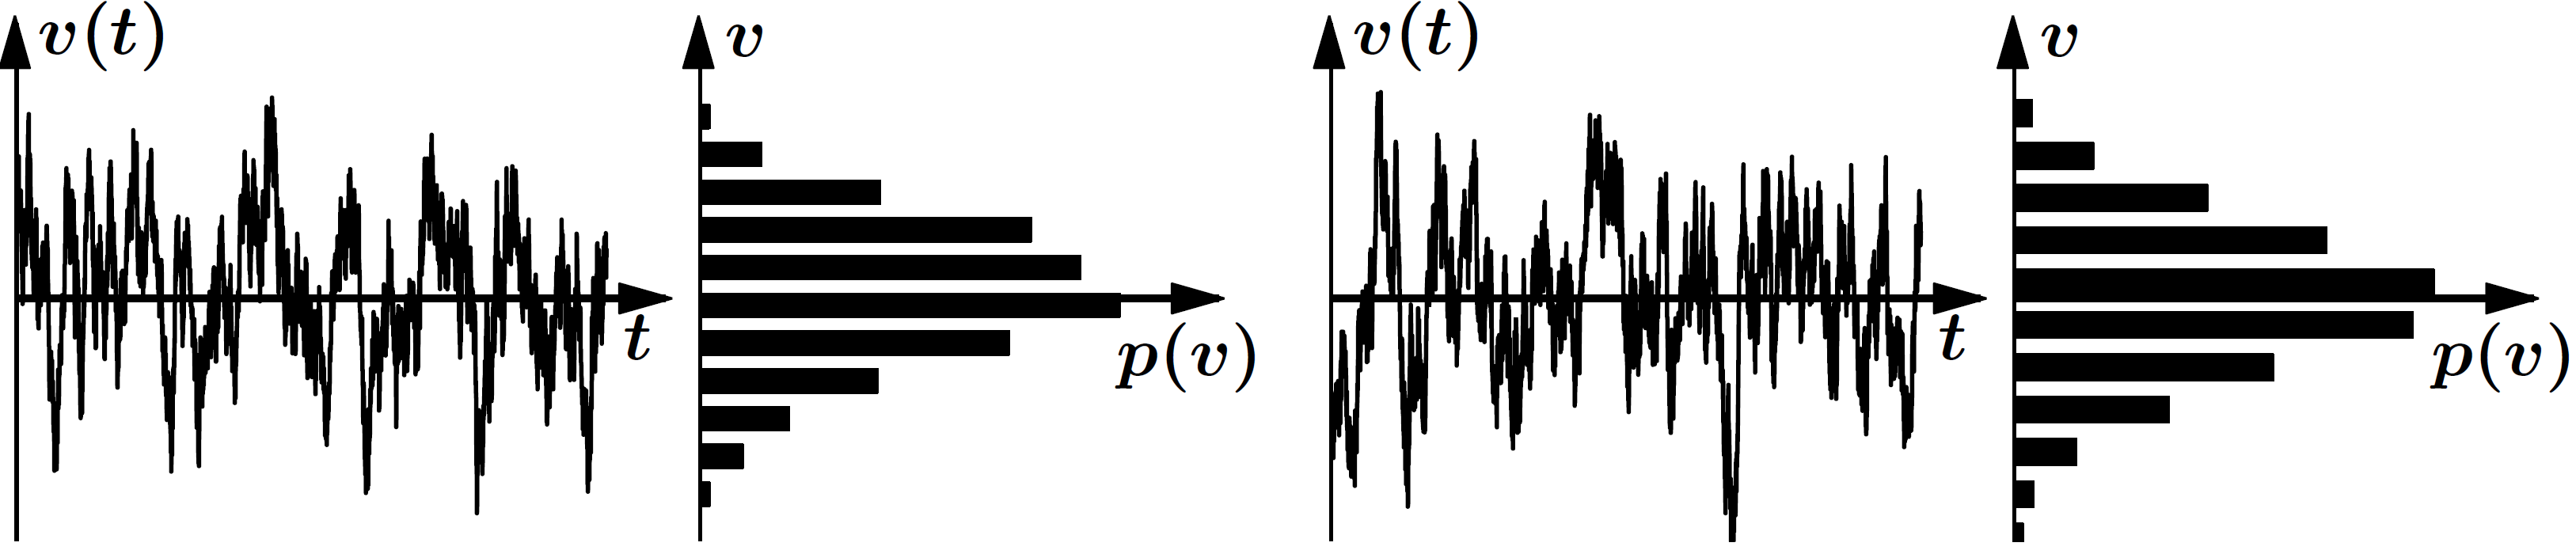
\includegraphics[width=\linewidth]{rss.png}
		\caption{Two realizations calculated from (\ref{eq:lesln})}
		\label{fig:rss}
	\end{subfigure}
	\vline
	\begin{subfigure}{0.35\linewidth}
		\centering
		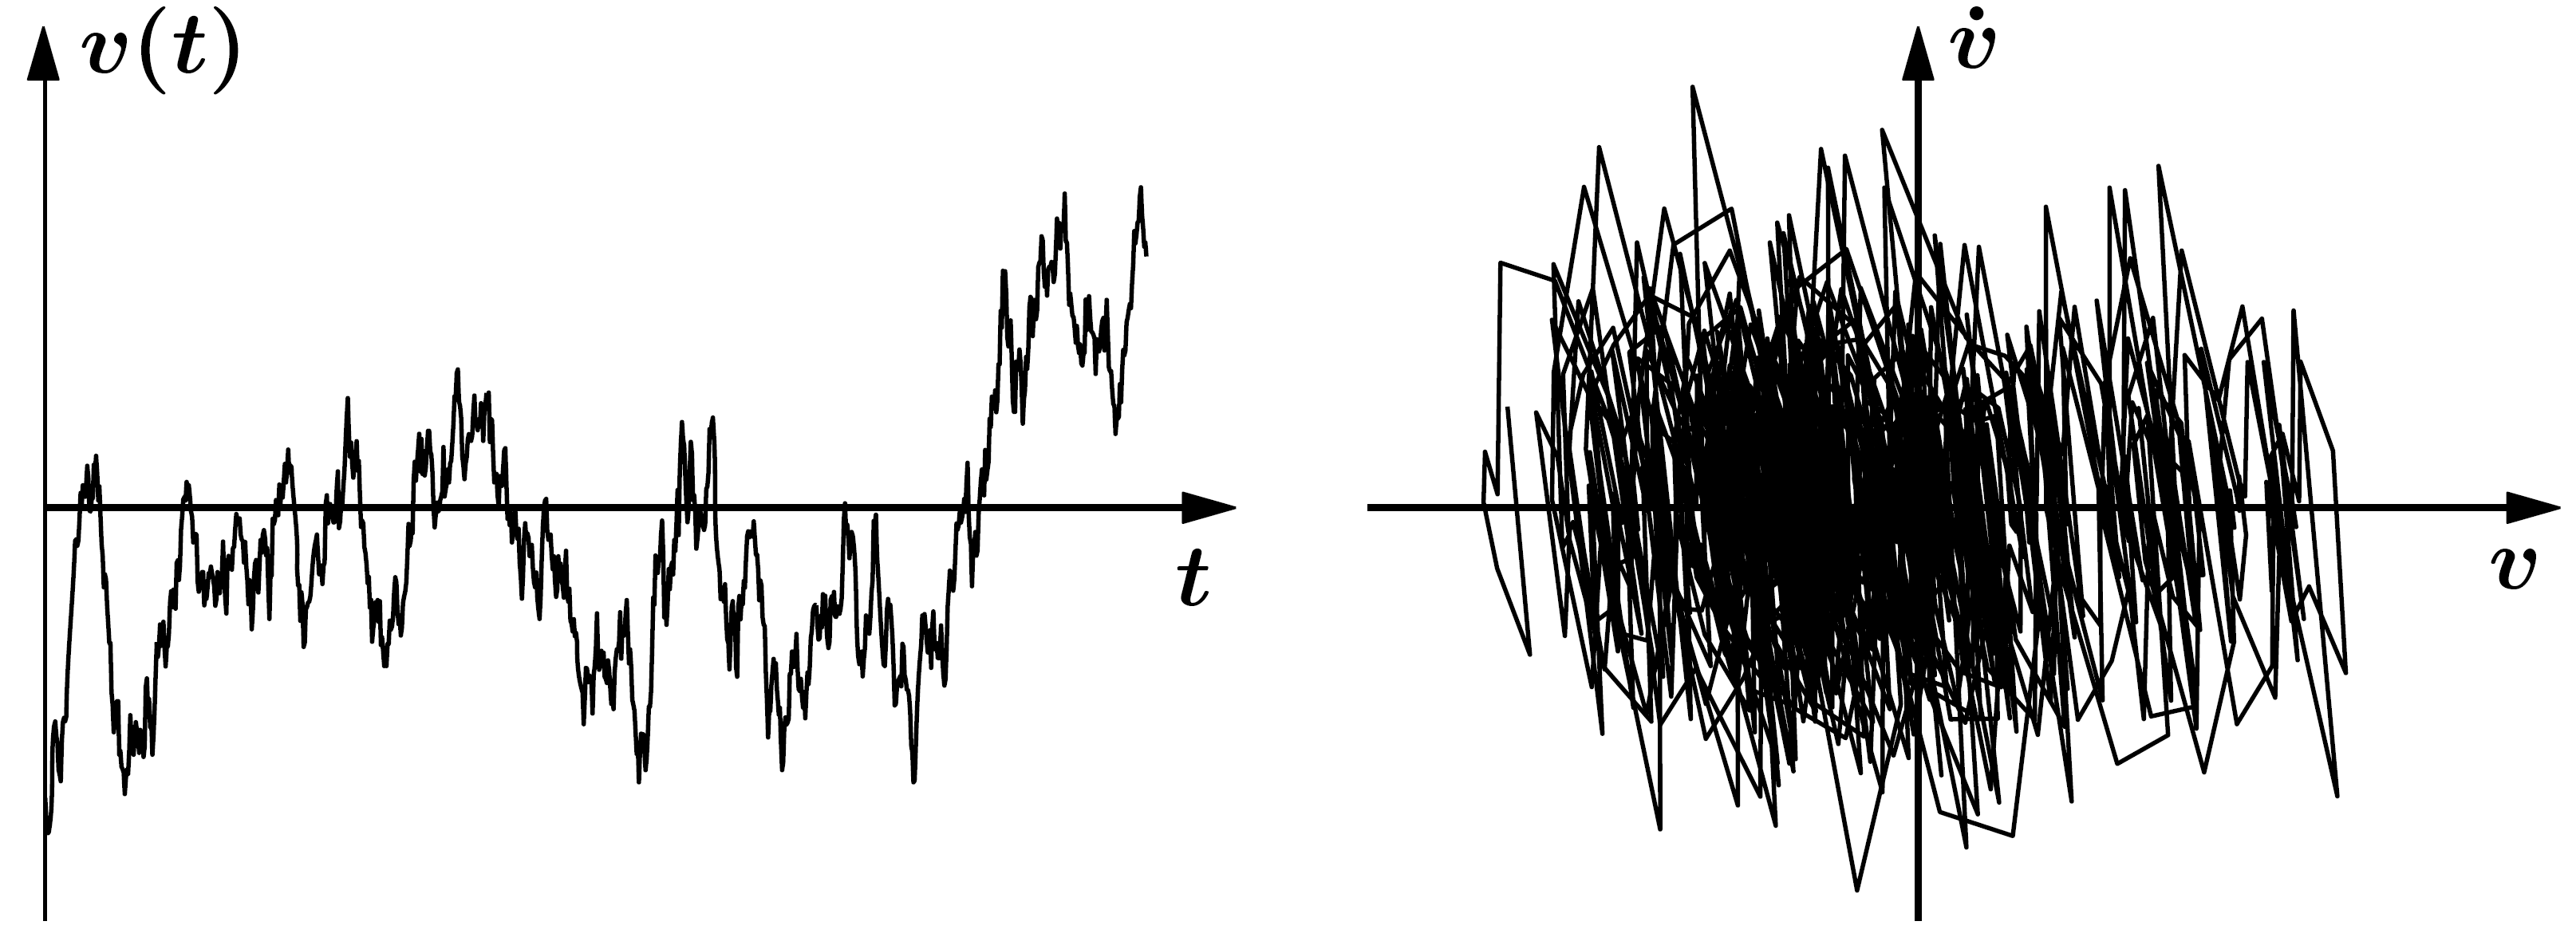
\includegraphics[width=\linewidth]{tspspss.png}
		\caption{Time series and phase space plot for a solution of (\ref{eq:bm2}).}
		\label{fig:tspspss}
	\end{subfigure}
\end{figure}
Two time series calculated from (\ref{eq:lesln}) are shown in Figure (\ref{fig:rss}), where the values for $\xi(t)$ were obtained from a random number generator.
Such different solutions of (\ref{eq:bm2}) are called \textbf{realizations} of the stochastic system.\\ Evidently, the time series are quite different, however the \emph{distributions} of the values in the time series, represented by the histograms, are very similar.
Such distributions are the foundation of stochastic systems.\\
In Figure (\ref{fig:tspspss}), without the stochastic term the trajectory would evolve to the stable fixed point $\tilde{v}=0$ but the stochastic force allows the system to explore its \emph{entire phase space}.
In contrast to deterministic systems, the trajectories in stochastic systems \emph{intersect}.